\documentclass{beamer}

\usepackage[english]{babel}
\usepackage{beamerthemeBoadilla}
%\usepackage{beamerthemeCambridgeUS}
%\usepackage{beamerthemeRochester}
%\usepackage{beamerthemeSzeged}
%\usepackage{beamerthemeMontpellier}
%\usepackage{beamerthemedefault}
\usepackage{url}
\usepackage{verbatim}
\usepackage[utf8]{inputenc}
\usepackage{multirow}
\usepackage{fancyvrb}
\usepackage{proof-dashed}
\newcommand{\mz}{\m{match} \;}
\newcommand{\stepz}{\m{step} \;}
\newcommand{\tab}[0]{\;\;\;\;}
\newcommand{\dz}{\m{derive}~}
\newcommand{\comp}[0]{\m{comp} \;}
\newcommand{\az}{\m{apply} \;}
\newcommand{\doz}{\m{run} \;}
\newcommand{\seqnocut}[3]{#1 ; #2 \Rightarrow #3}
\newcommand{\defeq}{\buildrel\triangle\over =}
\newcommand{\compr}[1]{\m{def} \; #1}

\newcommand{\stepo}{\m{step}_{LLD} \;}
\newcommand{\mo}{\m{match}_{LLD} \;}
\newcommand{\contlld}{\m{cont}_{LLD}}
\newcommand{\cont}{\contlld \;}
\newcommand{\contclld}{\m{cont}_{LLDc}}
\newcommand{\contc}{\contclld \;}
\newcommand{\done}{\m{derive}_{LLD} \;}
\newcommand{\doo}{\m{run}_{LLD} \;}
\newcommand{\matchlldc}{\m{match}_{LLDc}}
\newcommand{\mc}[0]{\matchlldc \; }
\newcommand{\dall}[0]{\m{fix}_{LLD} \; }
\newcommand{\strans}[0]{\m{update}_{LLD} \;}
\newcommand{\dc}{\m{derive}_{LLDc} \;}
\newcommand{\ao}{\m{apply}_{LLD} \;}

\newcommand{\com}{\xrightarrow{*}}
%\mapsto}
\newcommand{\feq}[2]{#1 \equiv #2}
\usepackage{latexsym}
\usepackage{amssymb}            % for \multimap (-o)
\usepackage{stmaryrd}           % for \binampersand (&), \bindnasrepma (\paar)

\newcommand{\m}[1]{\mathsf{#1}}
\newcommand{\f}[1]{\framebox{#1}}

\newcommand{\eph}{\mathit{eph}}
\newcommand{\pers}{\mathit{pers}}
\newcommand{\um}[1]{\underline{\m{#1}}}

\newcommand{\seq}{\vdash}
\newcommand{\semi}{\mathrel{;}}
\newcommand{\lequiv}{\mathrel{\dashv\vdash}}

% symbols of linear logic
\newcommand{\lolli}{\multimap}
\newcommand{\tensor}{\otimes}
\newcommand{\with}{\mathbin{\binampersand}}
\newcommand{\paar}{\mathbin{\bindnasrepma}}
\newcommand{\one}{\mathbf{1}}
\newcommand{\zero}{\mathbf{0}}
\newcommand{\bang}{{!}}
\newcommand{\whynot}{{?}}
\newcommand{\bilolli}{\mathrel{\raisebox{1pt}{\ensuremath{\scriptstyle\circ}}{\lolli}}}
% \oplus, \top, \bot



\newsavebox{\mysavebox}

\def\Tiny{\fontsize{6pt}{6pt}\selectfont}

\title{Design and Implementation of a Multithreaded Virtual Machine for Executing Linear Logic Programs}
\author[Flávio Cruz]{Flávio Cruz {\small \texttt{<fmfernan@cs.cmu.edu>}}\\
\scriptsize{\textbf{Authors}:\\
Flavio Cruz (CMU/UP)\\
Ricardo Rocha (UP)\\
Seth Goldstein (CMU)}}

\institute[CMU/UP]{Carnegie Mellon University \\ Pittsburgh, PA 15213, USA \and
CRACS \& INESC TEC, Faculty of Sciences, University Of Porto\\
Rua do Campo Alegre, 1021/1055, 4169-007 Porto, Portugal}
\date{\today}

\let\oldalert\alert
\renewcommand{\alert}[2][]{%
  \if\relax\detokenize{#1}\relax% http://tex.stackexchange.com/q/53068/5764
    \oldalert{#2}% Default overlay
  \else
    \oldalert<#1>{#2}% Specific overlay
  \fi}

\begin{document}

\frame{\titlepage}

\AtBeginSection[] { \begin{frame}<beamer>
\frametitle{Plan} \tableofcontents[currentsection]
\end{frame}}

\section{Introduction}

\frame
{
  \frametitle{Logic and Parallel Programming}
  \begin{itemize}
     \item Logic programs are declarative and easier to parallelize than imperative programs
     \begin{itemize}
      \item Logic program: set of rules
      \item Rules can be explored in parallel
      \item Imperative programming enforces a specific sequence of execution
     \end{itemize}
     \item Two paradigms:
     \begin{itemize}
      \item Backwards-chaining: Prolog
      \begin{itemize}
         \item Or-parallelism
         \item And-parallelism
      \end{itemize}
      \item Forwards-chaining: Datalog, \textbf{Linear Meld (LM)}
     \end{itemize}
  \end{itemize} 
}

\frame
{
   \frametitle{Forward Chaining Logic Programming}
   \begin{itemize}
      \item We start with a set of rules and a database of logical facts
      \item The database of facts is used to apply more rules
      \item Program stops when no more information can be derived
      \item Datalog: since all facts are persistent, concurrent rule application is trivial
      \item However, Datalog falls short when trying to express more stateful programs
   \end{itemize}
}

\subsection{Linear Meld}

\frame
{
   \frametitle{Linear Meld}
   \begin{itemize}
      \item Linear Meld (LM) is a Datalog-like language that incorporates Linear Logic
      \begin{itemize}
         \item Two kinds of facts: persistent facts and linear facts
         \item Linear facts can be retracted
      \end{itemize}
      \item Fully declarative language without extra-logical features
      \item LM programs are represented as a graph data structure
      \begin{itemize}
         \item Logical facts reside on a node of the graph
         \item Rules are locally restricted so that only node facts are manipulated
         \item No synchronization problems
      \end{itemize}
      %\item For a more in-depth view read our ICLP paper "A Linear Logic Programming Language for Concurrent Programming over Graph Structures"
   \end{itemize}
}

\subsection{Example}

\begin{frame}[fragile]
  \frametitle{Bipartiteness Checking}
  \begin{columns}[t]
     \column{.45\textwidth}
     \begin{block}{Program}
       \begin{Verbatim}[fontsize=\tiny,commandchars=\\\{\},frame=single]
\alert[1]{type route edge(node, node).}
\alert[1]{type linear mark(node, int).}
\alert[1]{type linear uncolored(node).}
\alert[1]{type linear colored(node, int).}
\alert[1]{type linear fail(node).}

fun next(int X) : int =
   if X <> 1 then 1 else 2 end.

\alert[2,6]{mark(@1, 1).}
\alert[2]{!edge(@1, @2). !edge(@1, @3).}
\alert[2]{!edge(@2, @4). !edge(@3, @4).}
\alert[2]{uncolored(A).}

\alert[3,7,8,9,10]{mark(A, P), uncolored(A)}
   \alert[3,7,8,9,10]{-o \{B | !edge(A, B) | mark(B, next(P))\},}
      \alert[3,7,8,9,10]{colored(A, P).}

\alert[4,11]{mark(A, P), colored(A, P)}
   \alert[4,11]{-o colored(A, P).}
\alert[5]{mark(A, P1), colored(A, P2), P1 <> P2}
   \alert[5]{-o fail(A).}
\alert[5]{mark(A, P), fail(A)}
   \alert[5]{-o fail(A).}
       \end{Verbatim}
     \end{block}
      \column{.5\textwidth}
      \begin{block}{\only<1>{Predicates}\only<2>{Axiom}\only<3>{First rule}\only<4>{Second rule}\only<5>{Third and fourth rule}\only<6-11>{Execution}}
         \centering
         {\scriptsize
         \only<1>{\begin{itemize}
                \item The first argument of every predicate must be typed as \texttt{node}.
                \item Predicates specified as \texttt{route} inform the compiler about the graph data structure.
                \item Predicates specified as \texttt{linear} turns facts of the predicate into linear facts, which can be asserted or retracted.
                \item Predicates not specified as \texttt{linear} are persistent.
                \item Nodes are either \texttt{colored/2} or \texttt{uncolored/1}.
             \end{itemize}}
         \only<2>{\begin{itemize}
                \item Axioms are rules without bodies that are added to the database as soon as the program starts.
                \item Node literals are written as \texttt{@X}, where \texttt{X} is the node number.
             \end{itemize}}
         \only<3>{\begin{itemize}
               \item If a node is scheduled to be \texttt{mark/1}'ed and is \texttt{uncolored/1}, then we can assign the color \texttt{P} to the node by deriving \texttt{colored(A,P)}.
               \item We use a comprehension to mark the neighbor nodes \\
               \texttt{\{B|!edge(A,B)|mark(B,next(P))\}}:
               \begin{itemize}
                  \item {\tiny For every \texttt{!edge(A, B)} in the database we derive a \texttt{mark(B,next(P))}.}
                  \item {\tiny With \texttt{next(P)} we attempt to color the neighbor node with the opposite color.}
               \end{itemize}
         \end{itemize}}
         \only<4>{\begin{itemize}
            \item If a node is to be marked with color \texttt{P} and has color \texttt{P}, then we keep it that way.
         \end{itemize}}
         \only<5>{\begin{itemize}
            \item However, if the colors are different then we derive \texttt{fail/1}.
            \item ... same if the coloring process has already failed.
         \end{itemize}}
         \only<6-11>{
         \begin{figure}[ht]
            \includegraphics<6>[height=4.5cm]{bipartiteness1.pdf}
            \includegraphics<7>[height=4.5cm]{bipartiteness2.pdf}
            \includegraphics<8>[height=4.5cm]{bipartiteness3.pdf}
            \includegraphics<9>[height=4.5cm]{bipartiteness4.pdf}
            \includegraphics<10>[height=4.5cm]{bipartiteness5.pdf}
            \includegraphics<11>[height=4.5cm]{bipartiteness6.pdf}
         \end{figure}
         }
      }
      \end{block}
  \end{columns}
\end{frame}

\section{Virtual Machine}

\begin{frame}[fragile]
   \frametitle{Virtual Machine}
   \begin{itemize}
      \item Register based machine implemented in C++
      \item Separate compiler compiles programs to byte-code
      \item Uses POSIX Threads for multithreading
      \item Optimized for:
      \begin{itemize}
         \item Parallelism
         \item Database storage and lookup of linear facts
         \item Fast rule execution
      \end{itemize}
   \end{itemize}
\end{frame}

\begin{frame}[fragile]
   \frametitle{Parallelism}
  \begin{columns}[t]
     \column{.45\textwidth}
{\small
      \begin{itemize}
      \item Graph is partitioned into P sub-graphs, where P is the number of threads
      \item Each thread processes the nodes of its sub-graph
      \item Work stealing is employed whenever threads start to starve
      \end{itemize}
}
     \column{.45\textwidth}
       \begin{block}{Partitioning}
       \begin{center}
          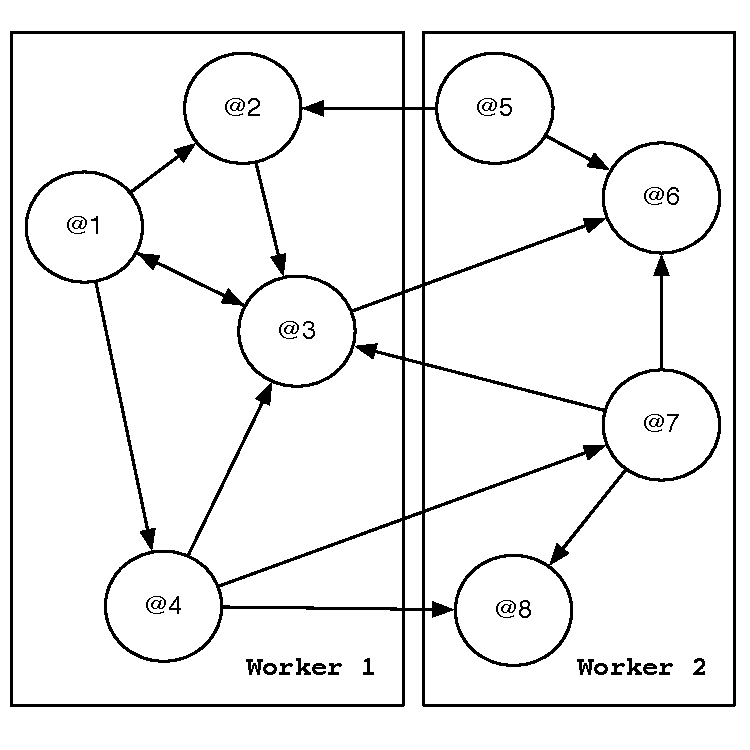
\includegraphics[height=5.5cm]{graph_coordination.pdf}
          \end{center}
       \end{block}
   \end{columns}
\end{frame}

\begin{frame}[fragile]
   \frametitle{Overview}
   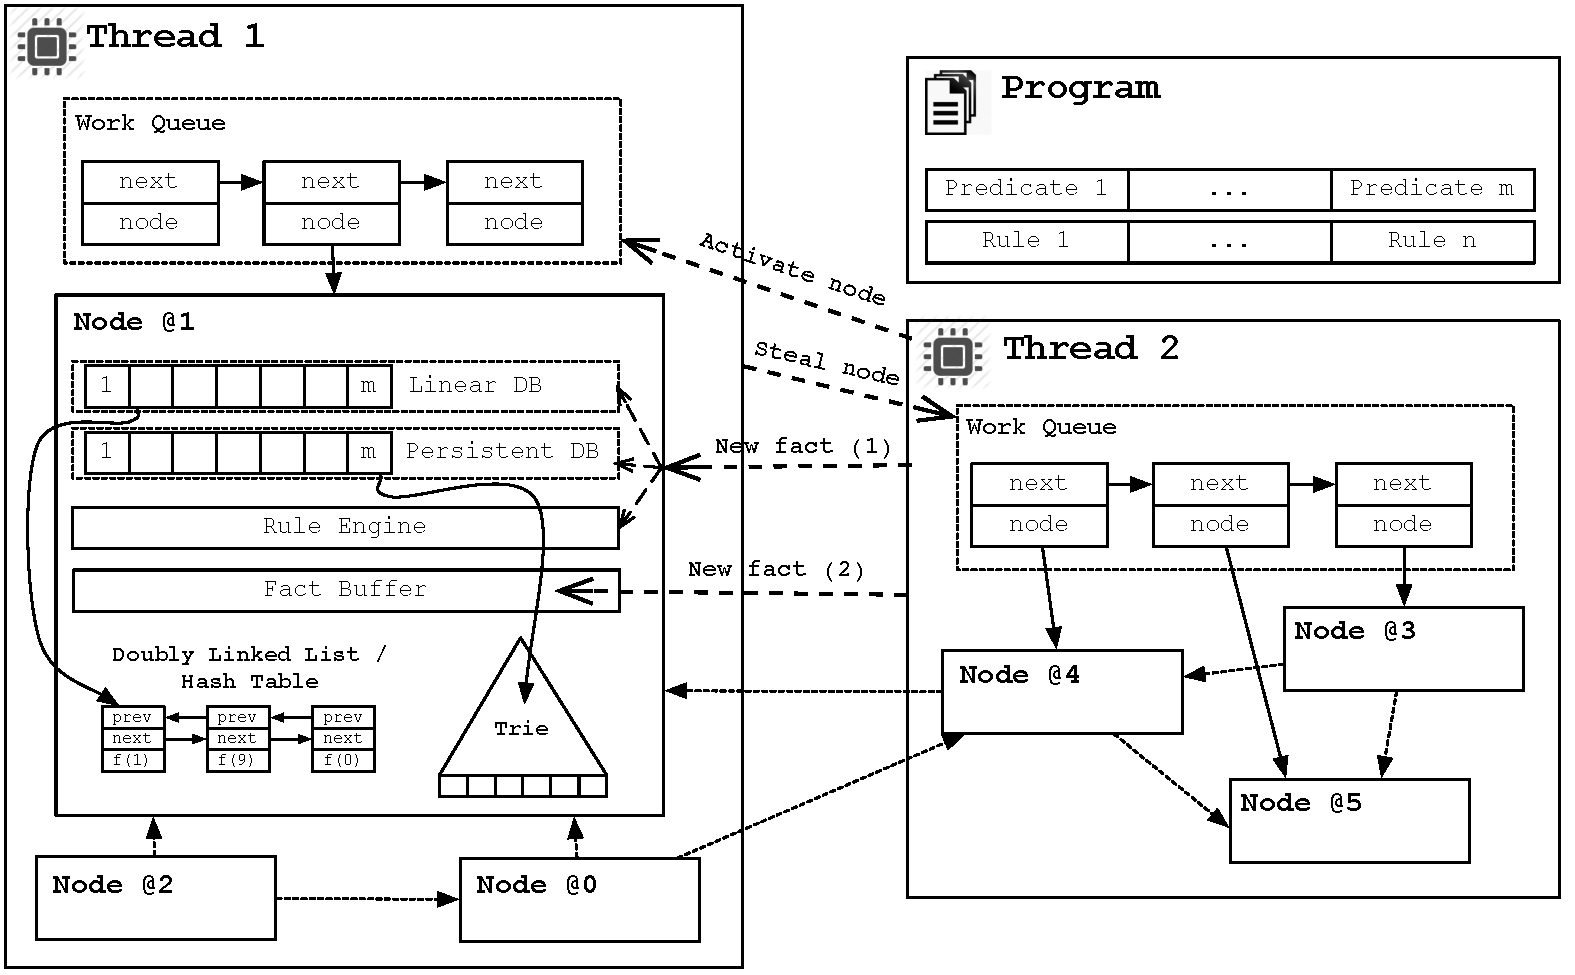
\includegraphics[height=7.5cm]{overview.pdf}
\end{frame}

\begin{frame}[fragile]
   \frametitle{Overview}
   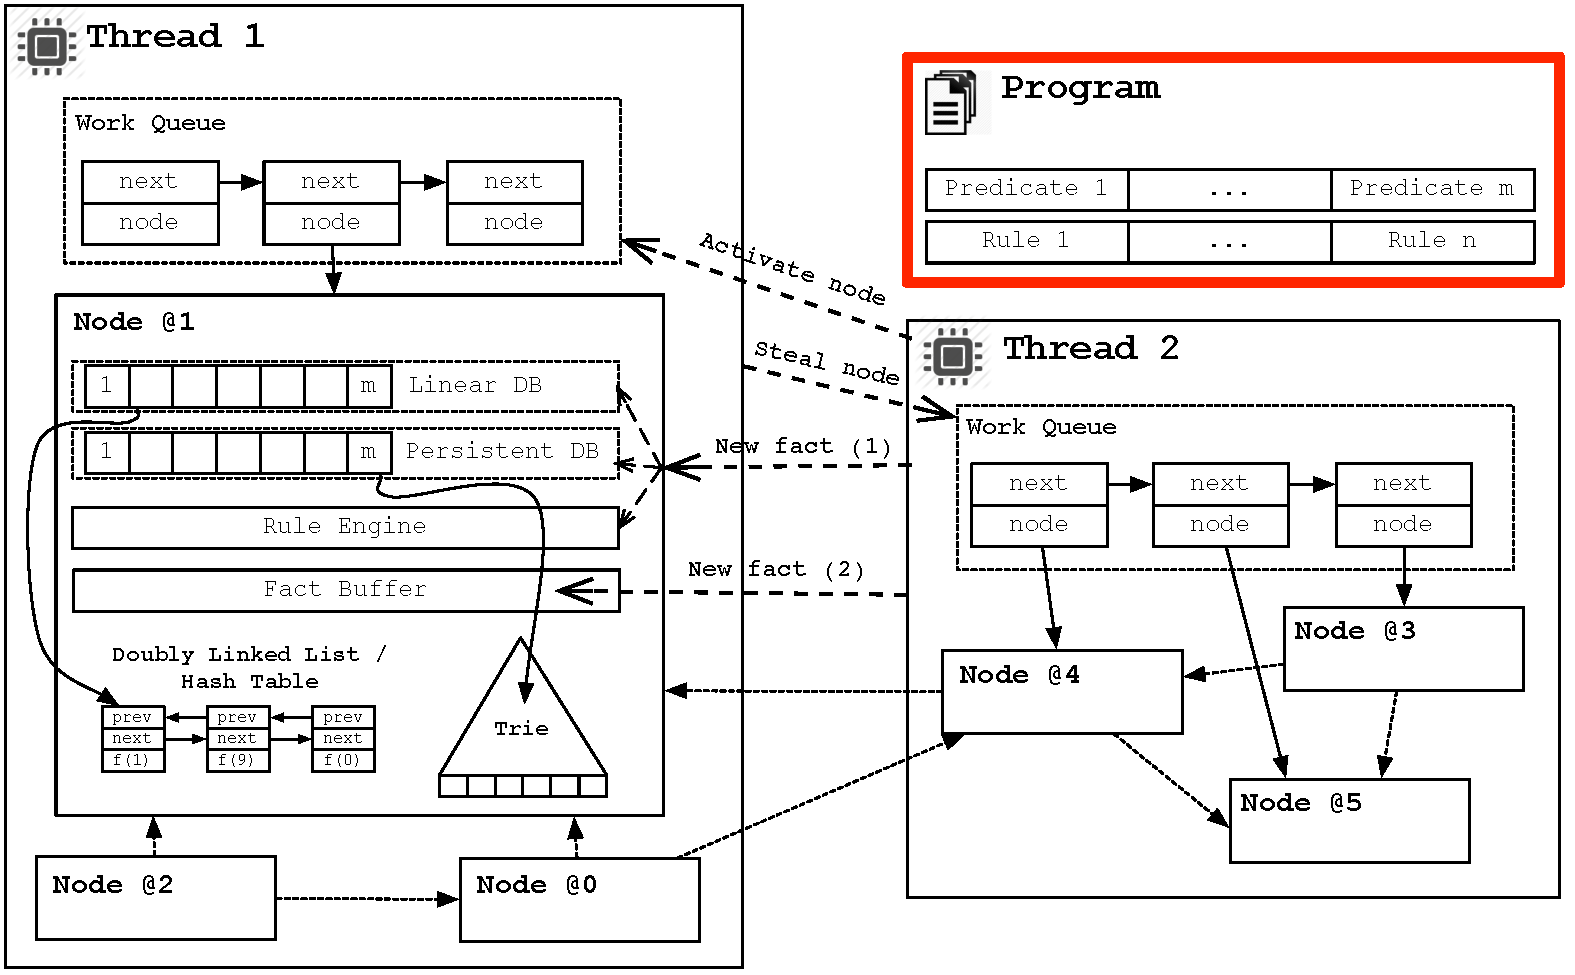
\includegraphics[height=7.5cm]{overview2.pdf}
\end{frame}

\begin{frame}[fragile]
   \frametitle{Byte Code}
   \begin{columns}[t]
   \column{.45\textwidth}
     \begin{block}{Program}
       \begin{Verbatim}[fontsize=\tiny,commandchars=\\\{\},frame=single]
type route edge(node, node).
type linear mark(node, int).
type linear uncolored(node).
type linear colored(node, int).
type linear fail(node).

fun next(int X) : int =
   if X <> 1 then 1 else 2 end.

mark(@1, 1).
!edge(@1, @2). !edge(@1, @3).
!edge(@2, @4). !edge(@3, @4).
uncolored(A).

\alert[1]{mark(A, P), uncolored(A)}
   \alert[1]{-o \{B | !edge(A, B) | mark(B, next(P))\},}
      \alert[1]{colored(A, P).}

mark(A, P), colored(A, P)
   -o colored(A, P).
mark(A, P1), colored(A, P2), P1 <> P2
   -o fail(A).
mark(A, P), fail(A)
   -o fail(A).
\end{Verbatim}
     \end{block}
   \column{.5\textwidth}
   \begin{block}{Byte Code}
\begin{Verbatim}[fontsize=\tiny]
LINEAR ITERATE OVER uncolored MATCHING TO reg 0
  LINEAR ITERATE OVER mark MATCHING TO reg 1
    ALLOC colored TO reg 2
    MVFIELDFIELD 1.0 TO 2.0
    ADDLINEAR reg 2
    RESET LINEAR
      PERSISTENT ITERATE OVER edge MATCHING TO reg 2
        ALLOC mark TO reg 3
        PUSH
        PUSH
        PUSH REGS
        MVFIELDREG 1.0 TO reg 0
        MVPCOUNTERSTACK TO STACK 33
        CALLF 0
        POP REGS
        MVSTACKFIELD STACK 0 TO 3.0
        POP
        POP
        MVFIELDREG 2.0 TO reg 4
        SEND reg 3 TO reg 4
        TRY NEXT
    END LINEAR
    REMOVE reg 1
    REMOVE reg 0
    TRY NEXT
  NEXT
\end{Verbatim}
   \end{block}
   \end{columns}
\end{frame}

\begin{frame}[fragile]
   \frametitle{Overview}
   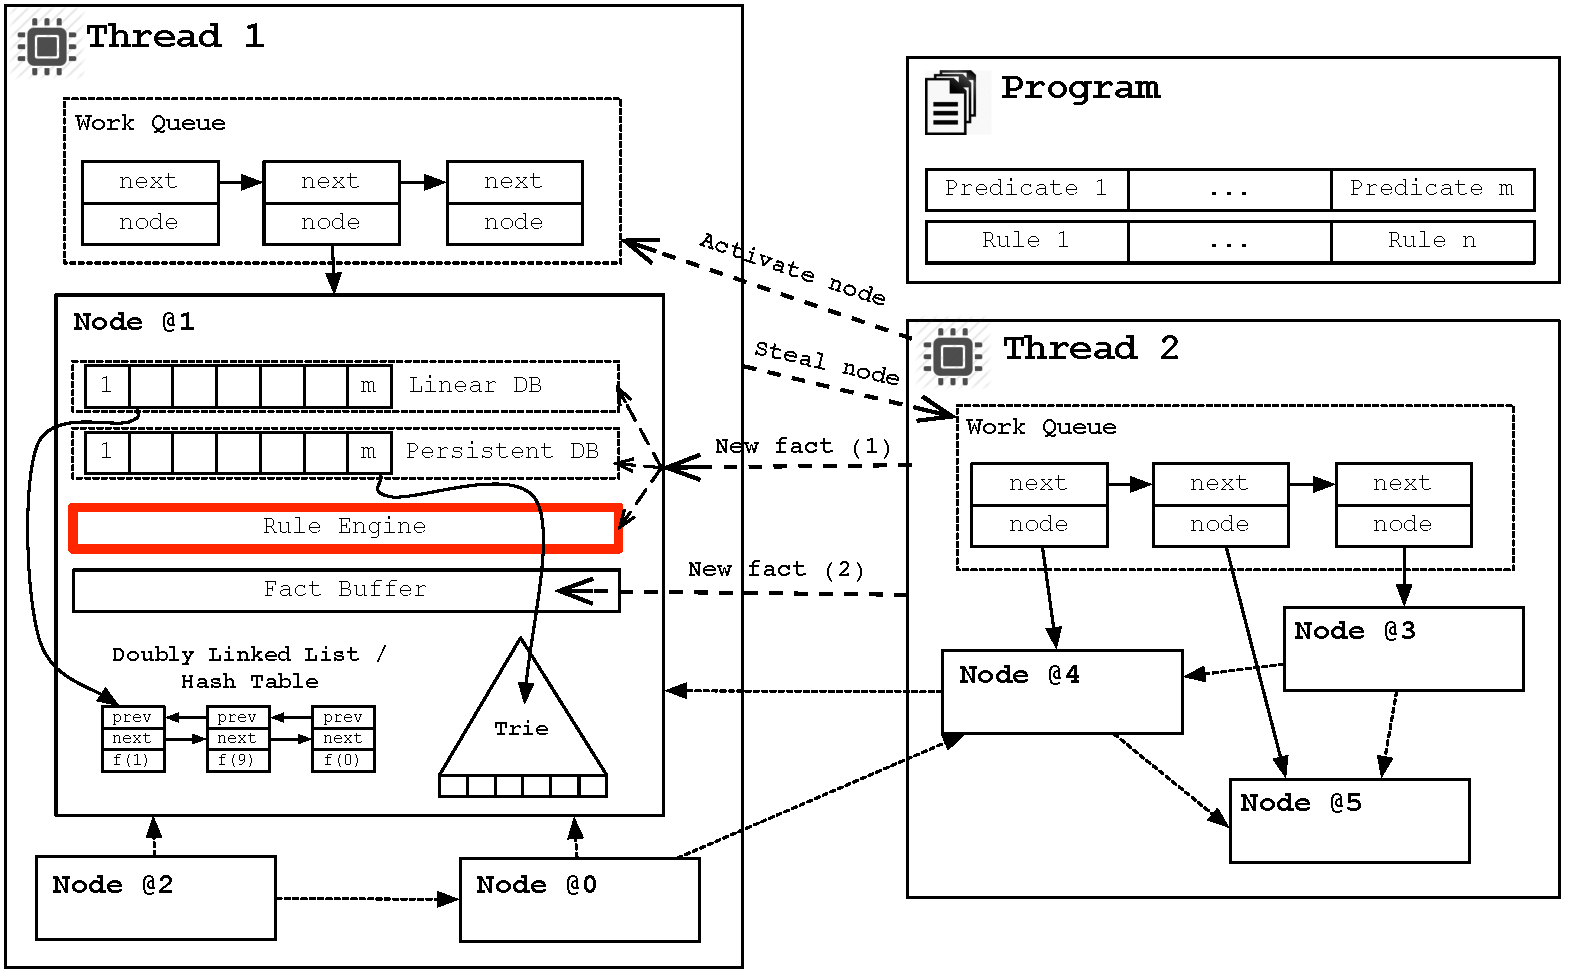
\includegraphics[height=7.5cm]{overview3.pdf}
\end{frame}

\begin{frame}[fragile]
   \frametitle{Rule Engine}
   \begin{itemize}
      \item Compact engine to detect which rules need to be executed (by priority)
      \item Structures:
      \begin{itemize}
         \item Predicates Count: compact bitmap to keep count of predicates
         \item Active Bitmap: rules "satisfied" with the current database
         \item Rule Queue: queue of rules to be executed
         \item Dropped Bitmap: rules that no longer are satisfied with the current database after a rule application
         \item Predicates Bitmap: bitmap of predicates/facts derived during a rule application.
      \end{itemize}
      \item How to update Rule Queue?
      \begin{itemize}
         \item Remove rules from Dropped Bitmap (XOR)
         \item Iterate through Predicates Bitmap and add all satisfied rules (Activate Bitmap) (OR)
      \end{itemize}
      \item Execute next rule? Get the least significant index
      \begin{itemize}
         \item \texttt{rule = FFS(rule\_queue)}
         \item \texttt{rule\_queue = rule\_queue \& (rule\_queue - 1)}
      \end{itemize}
   \end{itemize}
\end{frame}

\begin{frame}[fragile]
   \frametitle{Overview}
   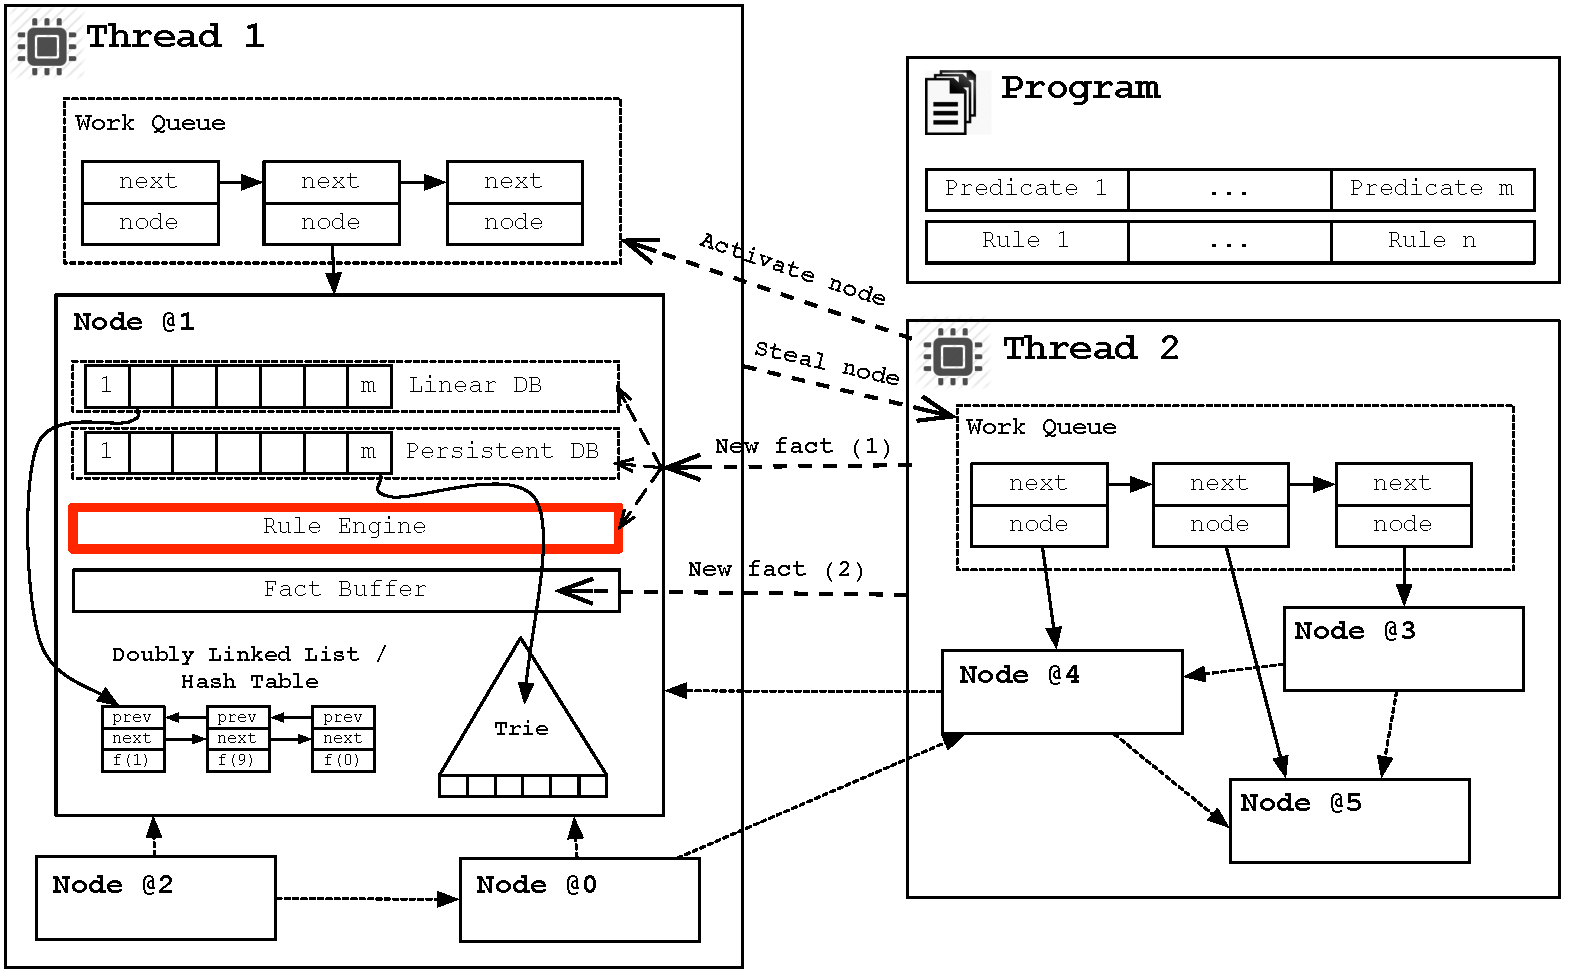
\includegraphics[height=7.5cm]{overview3.pdf}
\end{frame}

\begin{frame}[fragile]
   \frametitle{Database Structures}
   \begin{itemize}
      \item Tries are used for storing persistent facts
      \item Doubly linked lists for linear facts
      \begin{itemize}
         \item $\mathcal{O}(1)$ retraction
         \item $\mathcal{O}(1)$ assertion
         \item $\mathcal{O}(N)$ lookup
      \end{itemize}
      \item Hash tables also used for linear facts
      \begin{itemize}
         \item Indexing of facts using one of the arguments
         \item $\mathcal{O}(1)$ retraction and assertion
         \item $\mathcal{O}(1)$ lookup on average
         \item Full dynamic support
      \end{itemize}
   \end{itemize}
\end{frame}

\begin{frame}[fragile]
   \frametitle{Storing linear facts}
   \begin{center}
      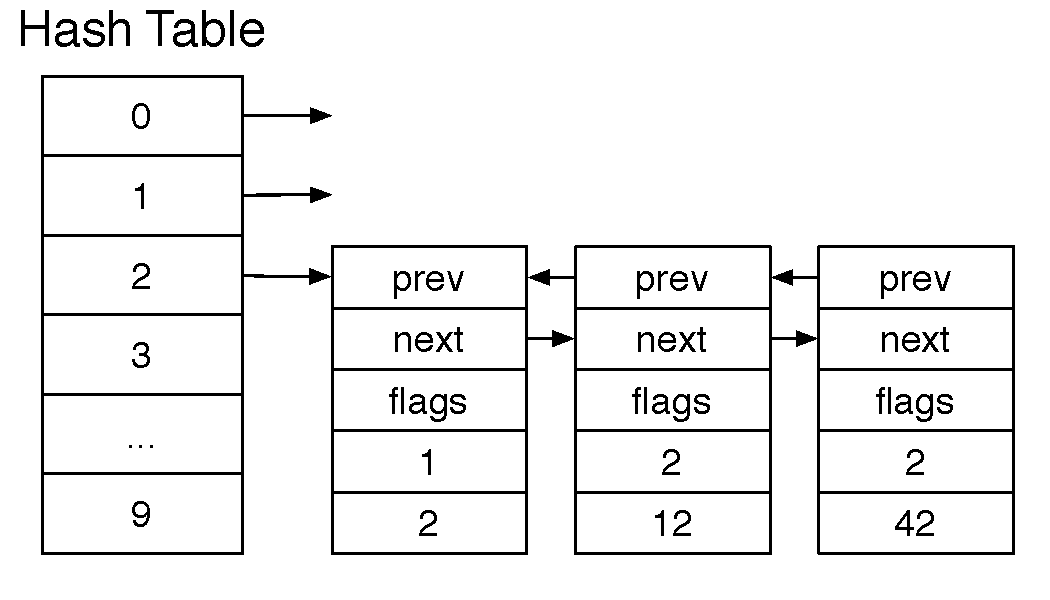
\includegraphics[height=6cm]{hash_table.pdf}
   \end{center}
   \begin{itemize}
      \item {\large Predicate \texttt{a(int, int)} indexed by the second argument}
   \end{itemize}
\end{frame}

\begin{frame}[fragile]
   \frametitle{Database Indexing}
   \begin{itemize}
      \item The virtual machine identifies during runtime the best indexing argument of each predicate
      \item Indexing algorithm is performed during the first few seconds of execution in 3 phases:
      \begin{itemize}
         \item Gathering of lookup data by keeping a counter for each argument
         \item Selecting the two best candidate arguments for each predicate
         \begin{itemize}
            \item If a predicate only uses 1 argument for lookup, then we use that argument
         \end{itemize}
         \item Compute entropy score for the two top arguments
      \end{itemize}
      \item Entropy: the more disorder there is for a given argument, the better
      \begin{itemize}
         \item The algorithm samples a few node databases to compute the entropy
      \end{itemize}
   \end{itemize}
\end{frame}


\section{Experimental Results}

\begin{comment}
\begin{frame}[fragile]
   \frametitle{Implemented programs}
   \begin{itemize}
      \item Belief Propagation
      \item MiniMax
      \item N-Queens
      \item PageRank
      \item Neural Networks
      \item Graph algorithms: shortest path, search, coloring
   \end{itemize}
\end{frame}
\end{comment}

\begin{frame}[fragile]
   \frametitle{Experimental Results: Scalability}
   \begin{columns}[t]
      \column{.5\textwidth}
      \begin{figure}[b]
         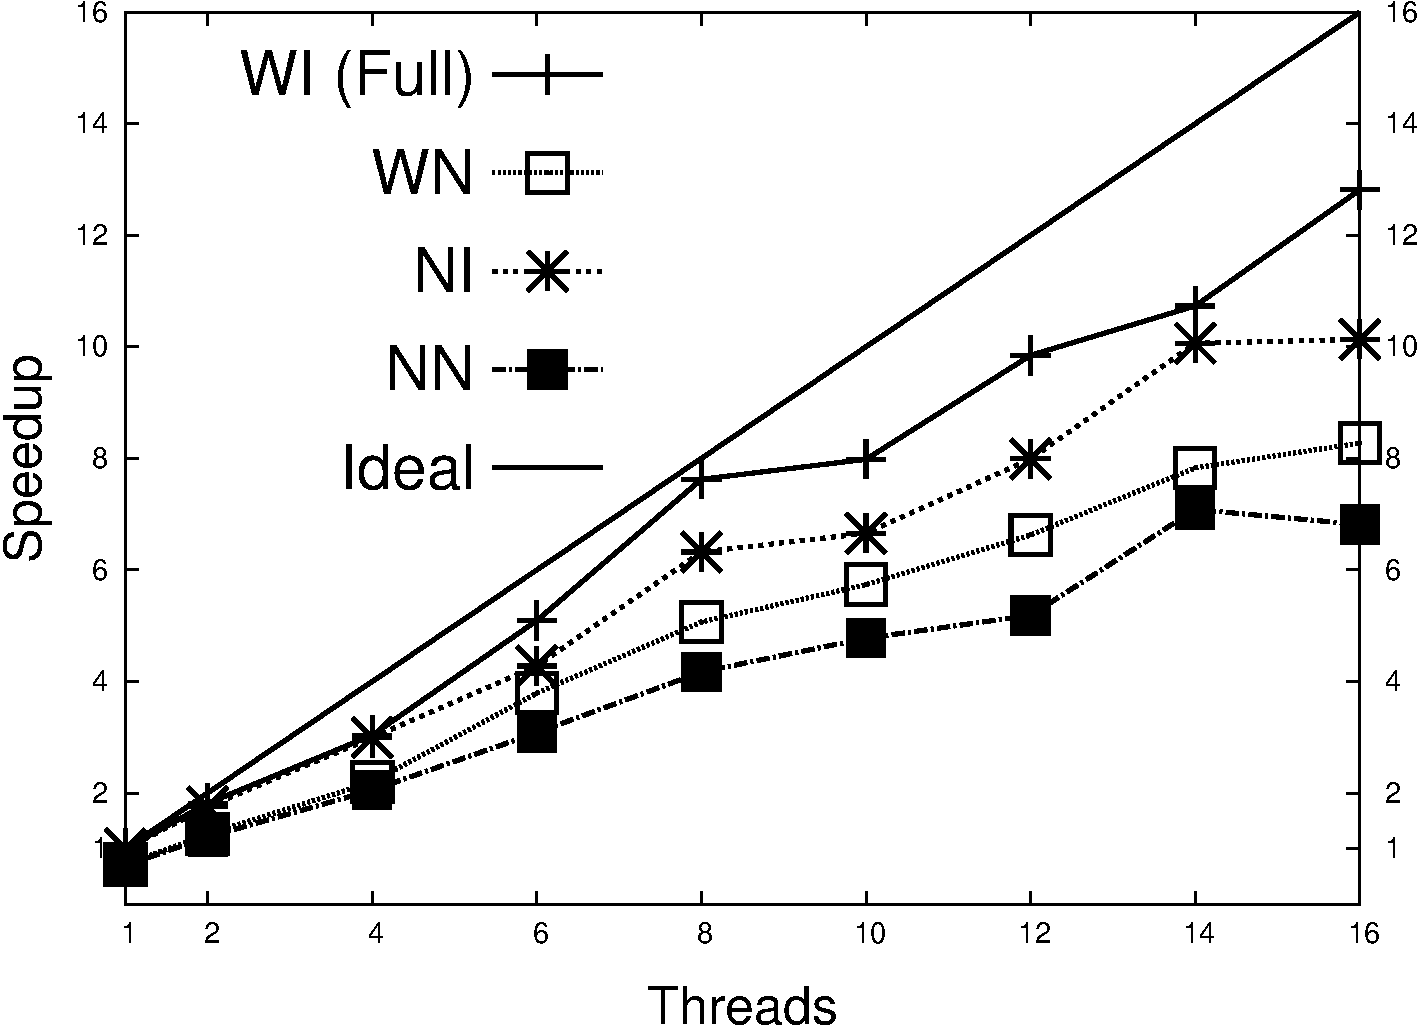
\includegraphics[width=\textwidth]{../figures/results-shortest-uspowergrid.pdf}
         \caption{Shortest Distance for a graph with around 5,000 nodes and 13,000 edges.}
      \end{figure}
      \column{.5\textwidth}
      \begin{figure}[b]
         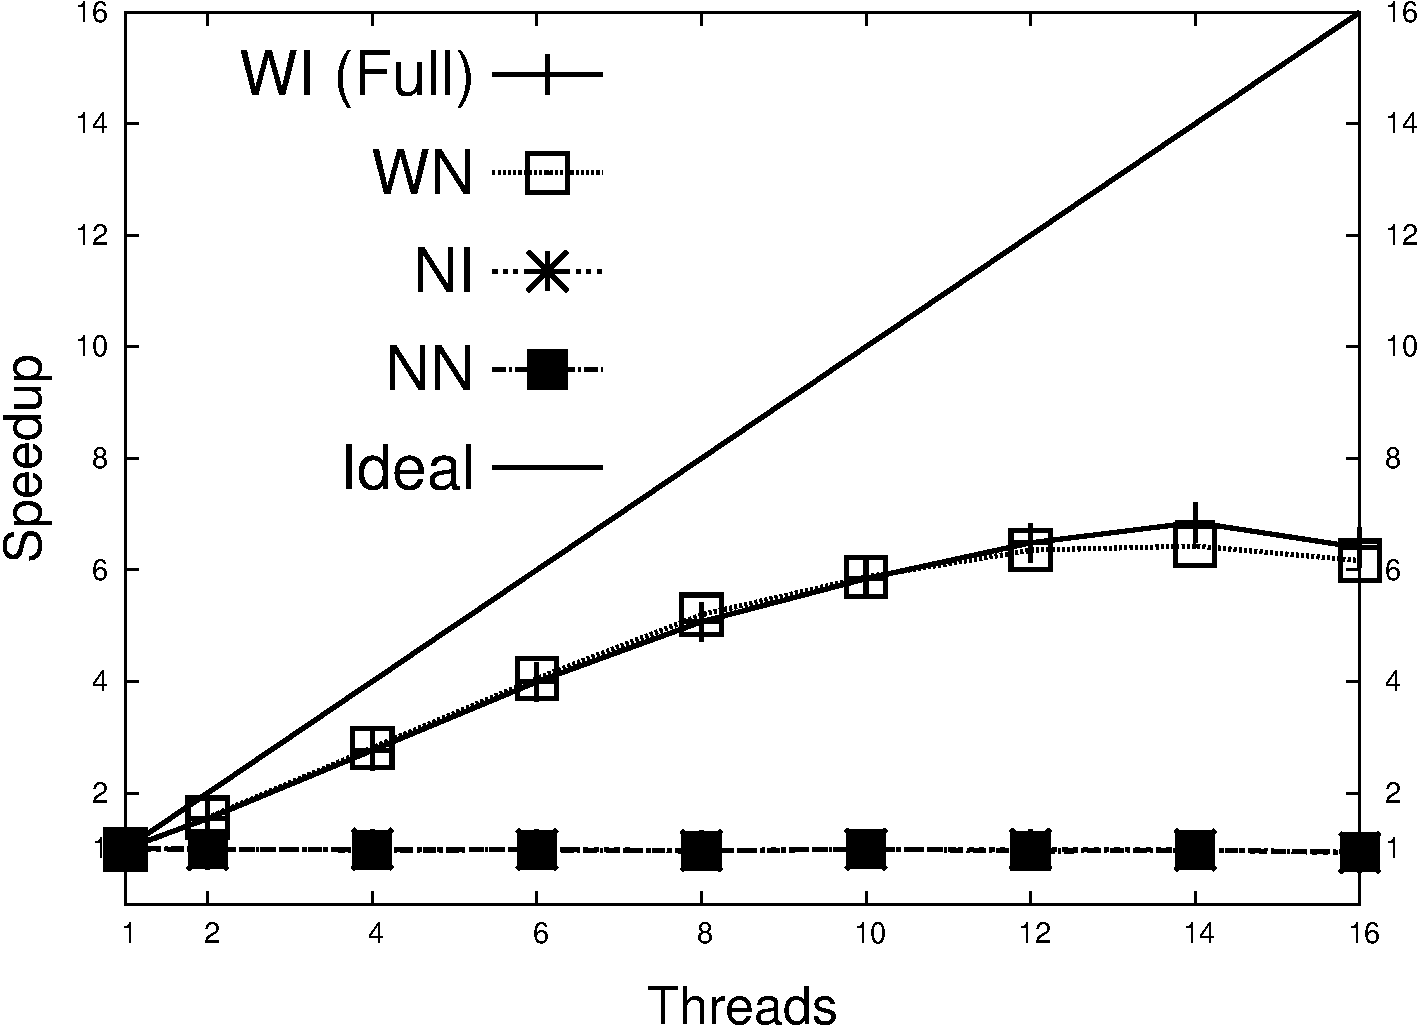
\includegraphics[width=\textwidth]{../figures/results-minimax.pdf}
         \caption{MiniMax algorithm for the Tic-Tac-Toe game.}
      \end{figure}
   \end{columns}
\end{frame}

\begin{frame}[fragile]
   \frametitle{Experimental Results: Scalability}
   \begin{columns}[t]
      \column{.5\textwidth}
      \begin{figure}[b]
         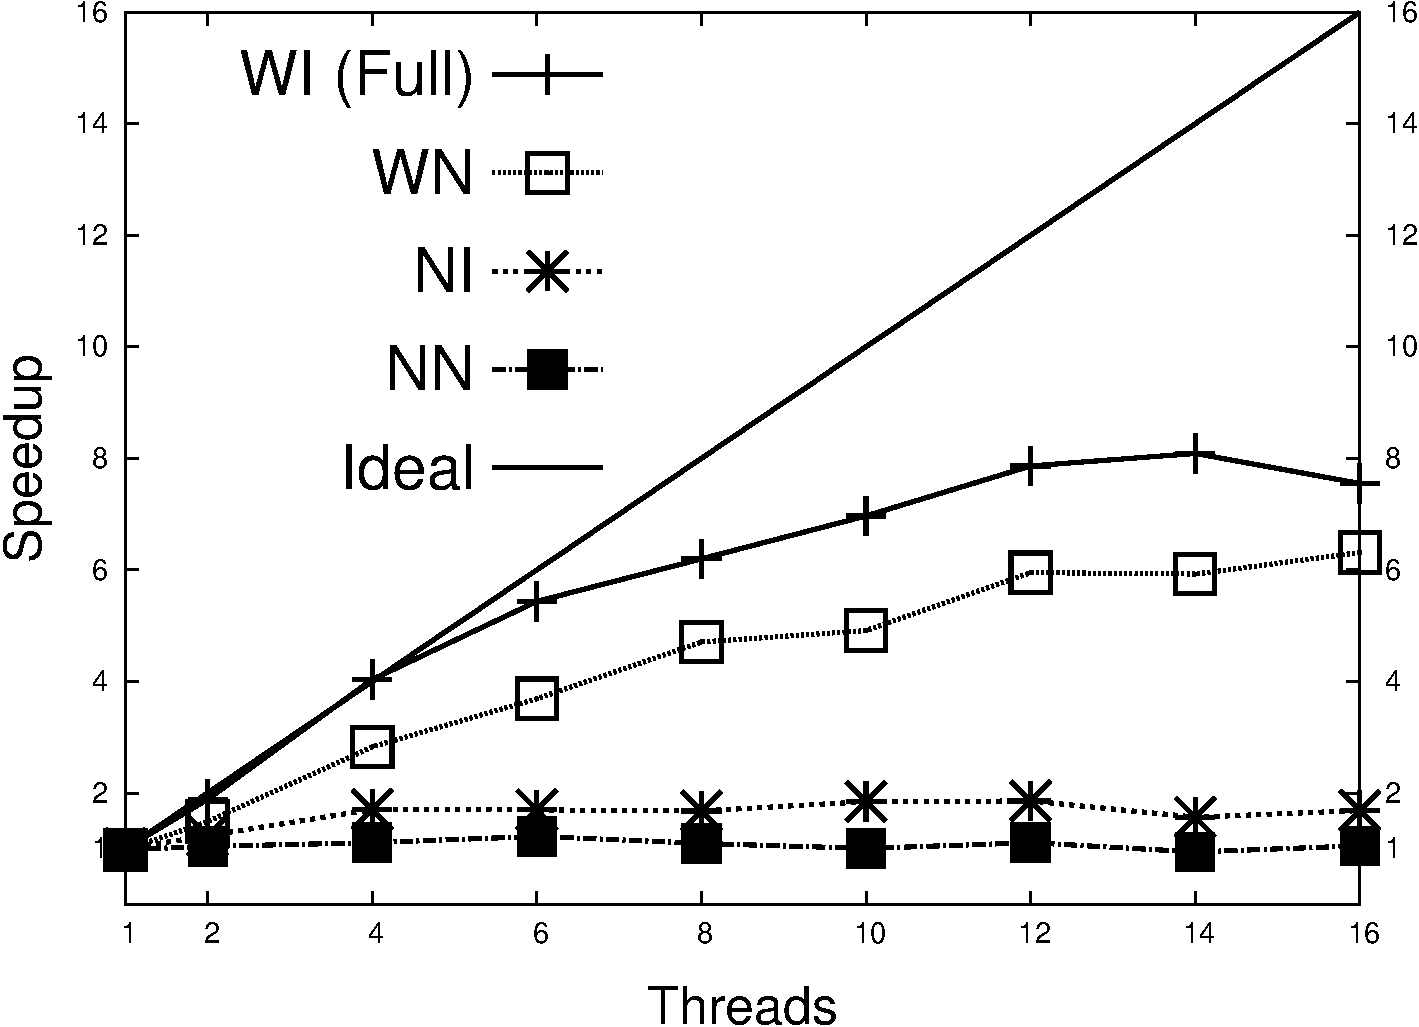
\includegraphics[width=\textwidth]{../figures/results-pagerank-search-engines.pdf}
         \caption{PageRank for a webpage graph.}
      \end{figure}
      \column{.5\textwidth}
      \begin{figure}[b]
         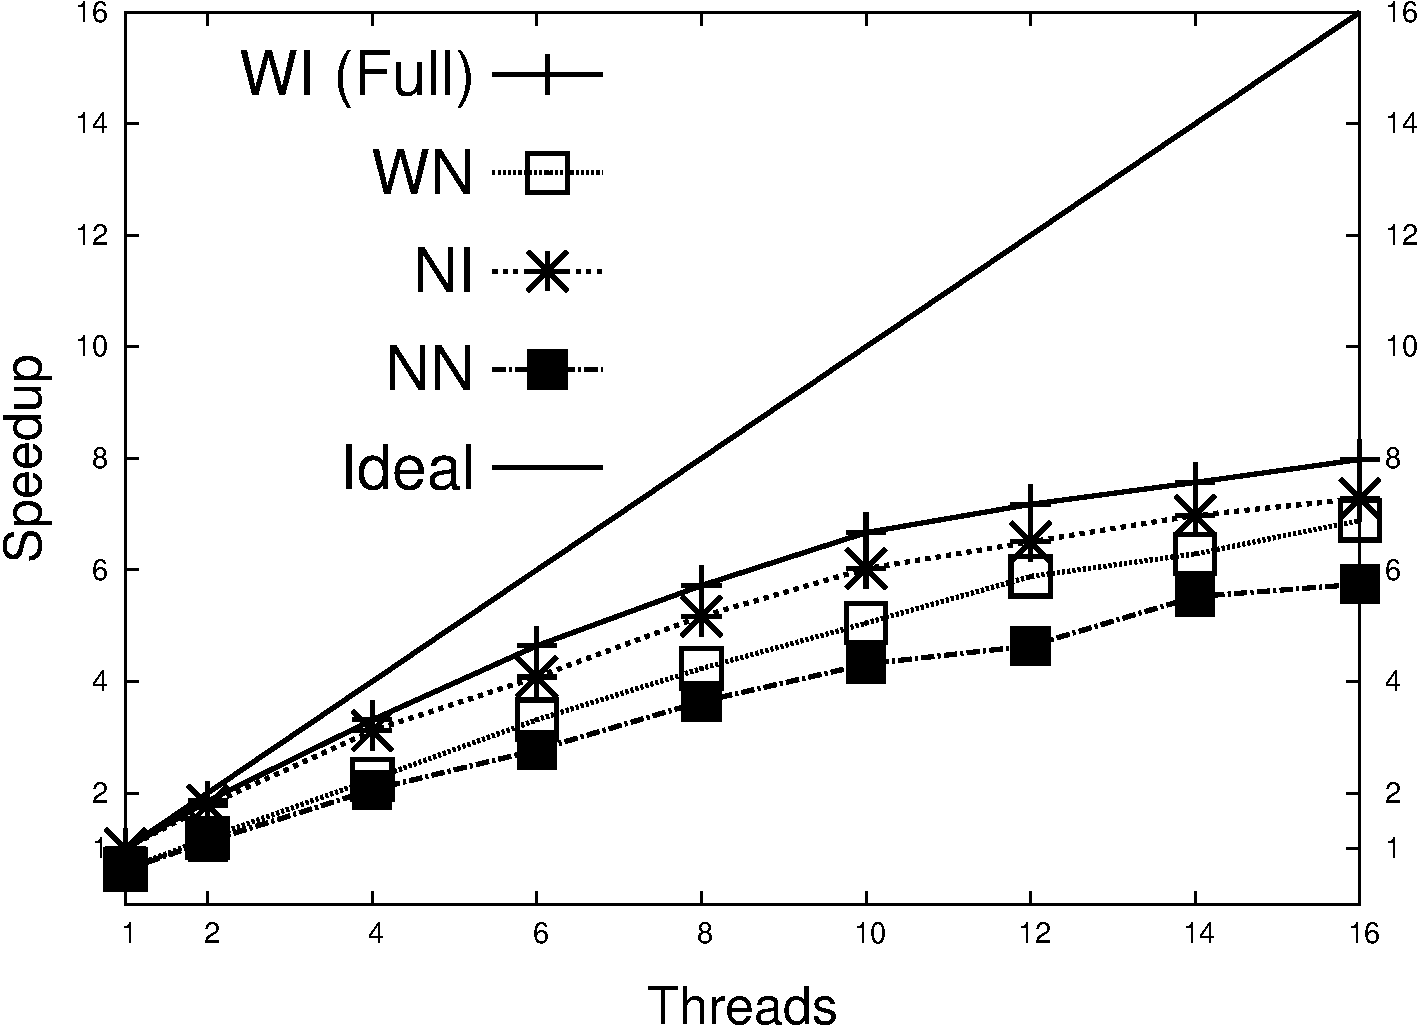
\includegraphics[width=\textwidth]{../figures/results-ggc.pdf}
         \caption{Greedy Graph Coloring for a random graph.}
      \end{figure}
   \end{columns}
\end{frame}

\begin{frame}[fragile]
   \frametitle{Experimental Results: Scalability}
   \begin{columns}[t]
      \column{.5\textwidth}
      \begin{figure}[b]
         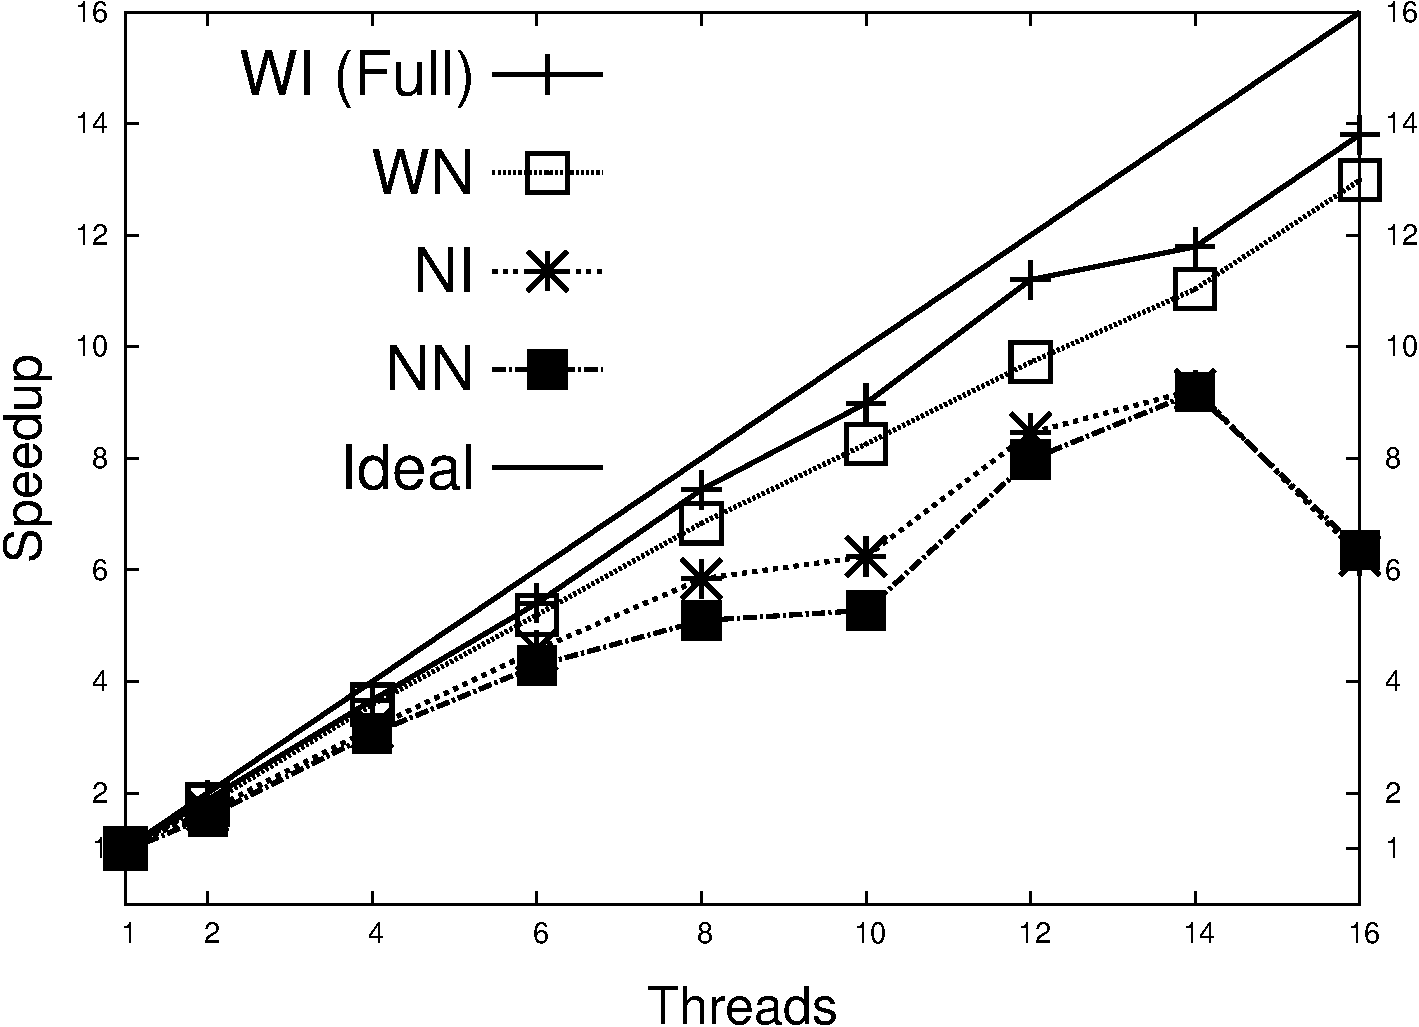
\includegraphics[width=\textwidth]{../figures/results-13queens.pdf}
         \caption{N-Queens program (13x13~board)}
      \end{figure}
      \column{.5\textwidth}
      \begin{figure}[b]
         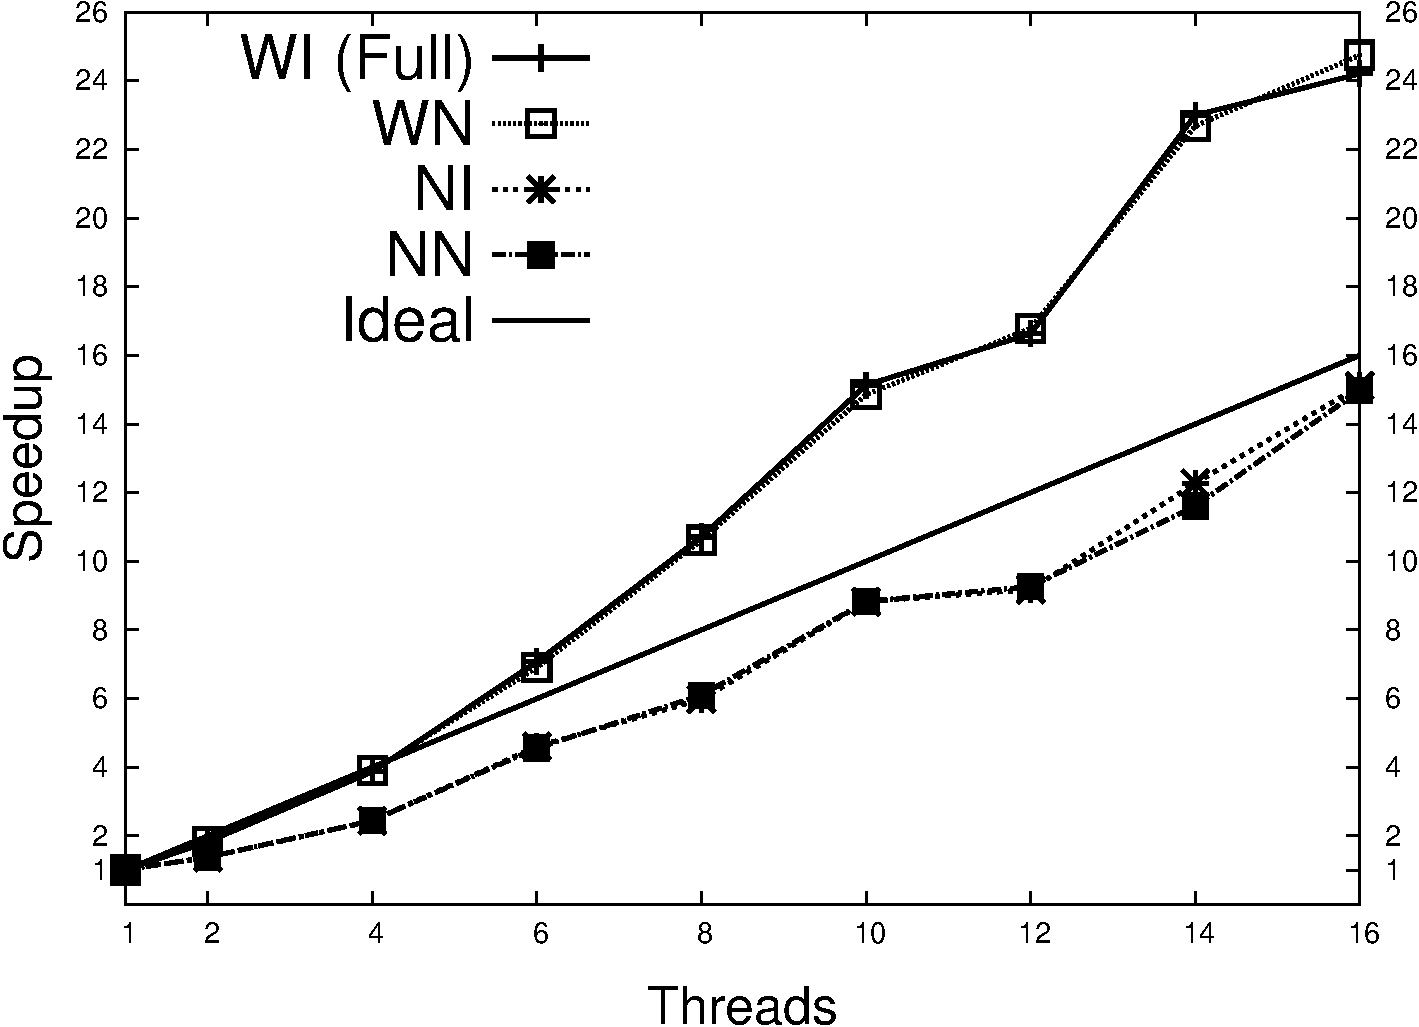
\includegraphics[width=\textwidth]{../figures/results-bp.pdf}
         \caption{Belief propagation (400x400 image).}
      \end{figure}
   \end{columns}
\end{frame}

\begin{frame}[fragile]
   \frametitle{Experimental Results: Absolute Execution Time}
   \begin{figure}[b]
      \begin{tabular}{ | l | l | l | l |}
       \hline
       Size & C & Python & YAP Prolog \\ \hline\hline
       10 & 16.92 & \textbf{0.62} & 5,42 \\
       11 & 21.59 & \textbf{0.64} & 6.47 \\
       12 & 10.32 & \textbf{0.73} & 7.61 \\
       13 & 14.35 & \textbf{0.88} & 10.38 \\
       \hline
       \end{tabular}
       \caption{N-Queens problem.}
    \end{figure}
    \begin{figure}[b]
       \begin{tabular}{ | l | l | l | l |}
        \hline

        Size & C & Python & GraphLab \\ \hline\hline
        10 & \textbf{1.00} & \textbf{0.03} & \textbf{1.00} \\
        50 & \textit{1.77} & \textbf{0.04} & \textit{1.73} \\
        200 & \textit{1.99} & \textbf{0.05} & \textit{1.79} \\
        400 & \textit{2.00} & \textbf{0.04} & \textit{1.80} \\
        \hline
        \end{tabular}
        \caption{Belief Propagation program.}
    \end{figure}
\end{frame}

\begin{frame}[fragile]
   \frametitle{Experimental Results: Memory Usage}
   \begin{center}
\begin{tabular}{c|c|c|c}
\textbf{Program} & \textbf{Facts} & \textbf{Memory} & \textbf{Per Fact} \\
\hline\hline
PageRank & 1,180,603 & 203,832 KB & 176 bytes \\
GGC & 2,363,536 & 292,682 KB & 127 bytes \\
SD & 502,347 & 45,387 KB & 92 bytes \\
MiniMax & 3 & 886,443 KB & 295,481 KB \\
N-Queens & 74,557 & 55,408 KB & 760 bytes \\
BP & 2,235,200 & 617,417 KB & 283 bytes \\
\hline\hline
\multicolumn{3}{l}{Average (without MiniMax) } & 288 bytes \\
\end{tabular}
\end{center}
\end{frame}

\begin{frame}
   \frametitle{Conclusions}
   \begin{itemize}
      \item LM programs are succinct
      \item The LM language is general enough to be ported to many distributed architectures
      \item The virtual machine aims to bridge the gap between logic programming and multicore technology
      \begin{itemize}
         \item Goal: execute large programs scalably and efficiently
      \end{itemize}
      \item Current work: use derivation rules to schedule computation
      \begin{itemize}
         \item Nodes have priority
         \item A given computation order will give the same result but will be complete faster
      \end{itemize}
   \end{itemize}
\end{frame}


\begin{frame}{Thank You}
\begin{center}
{\Huge Thank you for your time!}
\end{center}
\end{frame}

\end{document}

